\documentclass{beamer}
\usepackage{relsize}
\usepackage{color}

\usepackage{listings}
\usetheme{CambridgeUS}
%\usepackage{beamerthemesplit} % new 
\usepackage{enumitem}
\usepackage{amsmath}                    % See geometry.pdf to learn the layout options. 
\usepackage{amsthm}                   % See geometry.pdf to learn the layout options. There 
\usepackage{amssymb}                    % See geometry.pdf to learn the layout options. 
\usepackage[utf8]{inputenc} 
\usepackage{graphicx}
\usepackage[english,bulgarian]{babel}

\lstset{language=C++,
                basicstyle=\ttfamily,
                keywordstyle=\color{blue}\ttfamily,
                stringstyle=\color{red}\ttfamily,
                commentstyle=\color{green}\ttfamily,
                morecomment=[l][\color{magenta}]{\#}
}

\newtheorem{mydef}{Дефиниция}[section]
\newtheorem{lem}{Лема}[section]
\newtheorem{thm}{Твърдение}[section]

\DeclareMathOperator{\restrict}{\upharpoonright}

\setitemize{label=\usebeamerfont*{itemize item}%
  \usebeamercolor[fg]{itemize item}
  \usebeamertemplate{itemize item}}

\setbeamercovered{transparent}



\begin{document}
\title[Увод в програмирането]{Наредби в масиви} 
\author{Калин Георгиев} 
\frame{\titlepage} 


\section{Вмъкване} 


\begin{frame}
\centerline{Подреждане (сортиране) на данни}
\end{frame}


\begin{frame}[fragile]
\frametitle{Постановка на задачата}
\begin{itemize}
  \item Вход: 10,20,15,0,50
  \item Изход: 0,10,15,20,50
\end{itemize}
\end{frame}


\begin{frame}
\centerline{Нареждане при вмъкване / insertion sort}
\end{frame}



\begin{frame}[fragile]
\frametitle{Нареждане при вмъкване / insertion sort}

%\vspace*{-120pt}
%\hspace*{-30pt}
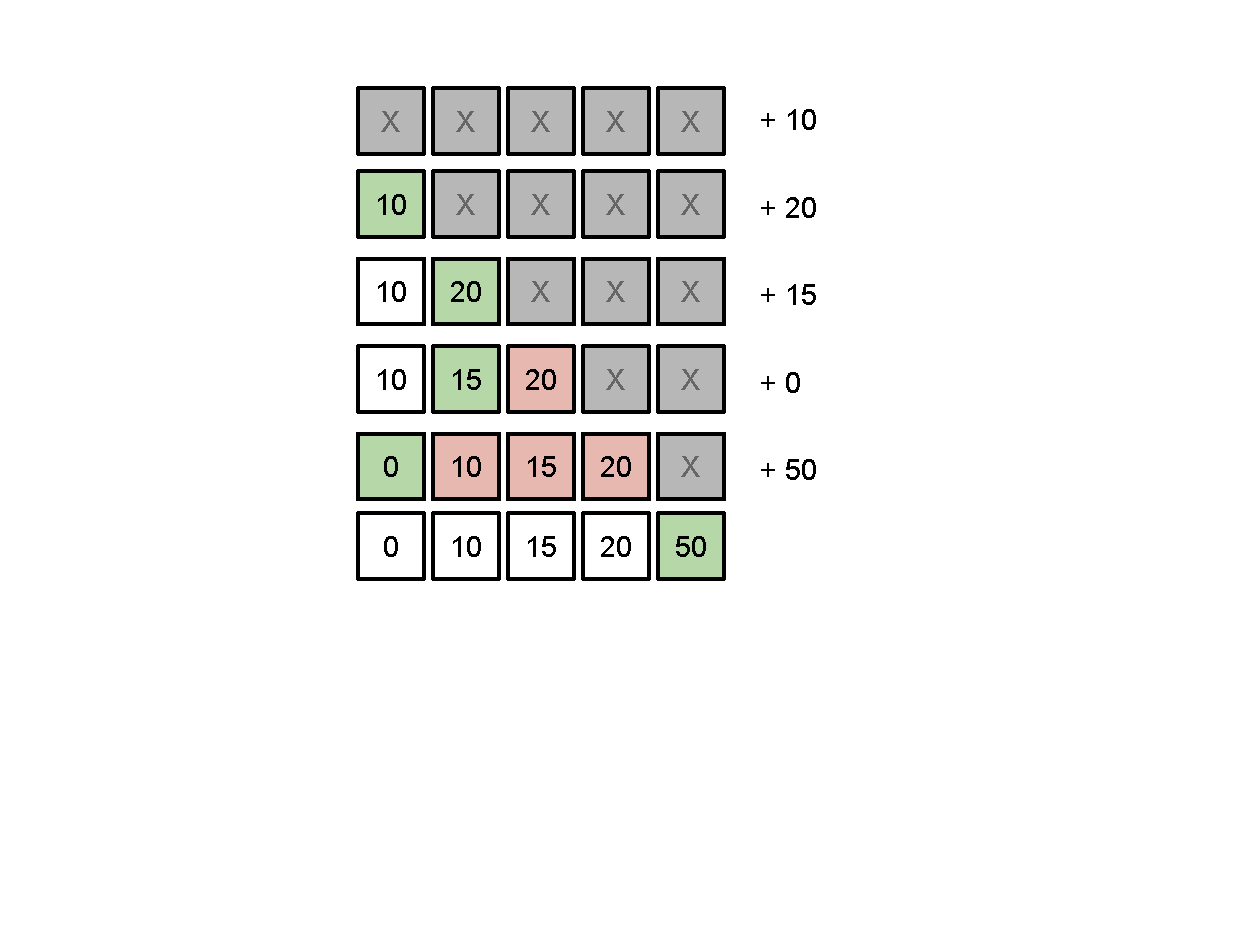
\includegraphics[width=14cm]{images/inssort} 

\end{frame}


\begin{frame}
\centerline{Намиране на най-малък елемент на масив}
\end{frame}



\begin{frame}[fragile]
\frametitle{Намиране на най-малък елемент на масив}

%\vspace*{-120pt}
\hspace*{-40pt}
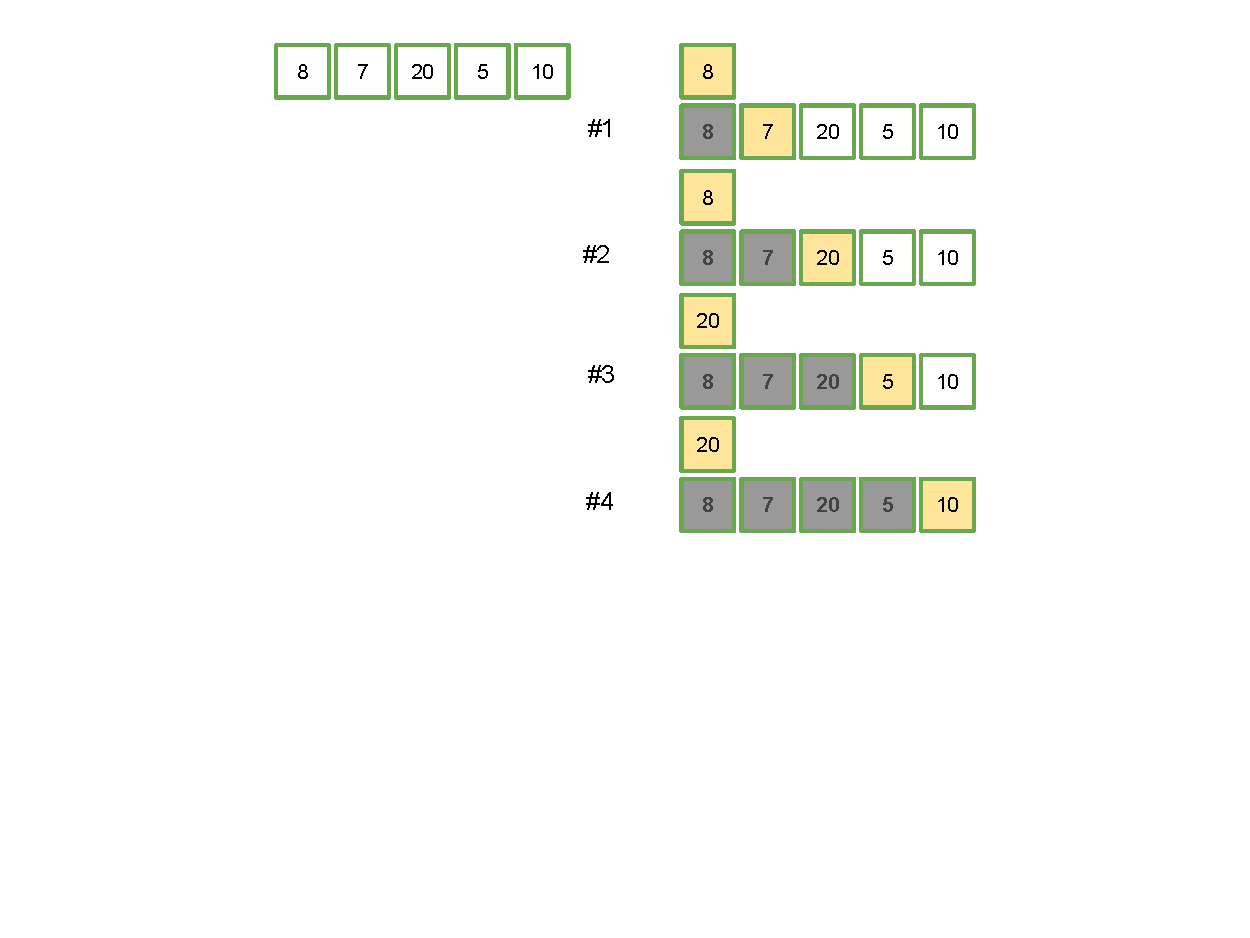
\includegraphics[width=14cm]{images/findmin} 

\end{frame}


\begin{frame}
\centerline{Сортиране чрез пряка селекция / straight selection sort}
\end{frame}



\begin{frame}[fragile]
\frametitle{Сортиране чрез пряка селекция / straight selection sort}


%\vspace*{-120pt}
%\hspace*{-40pt}
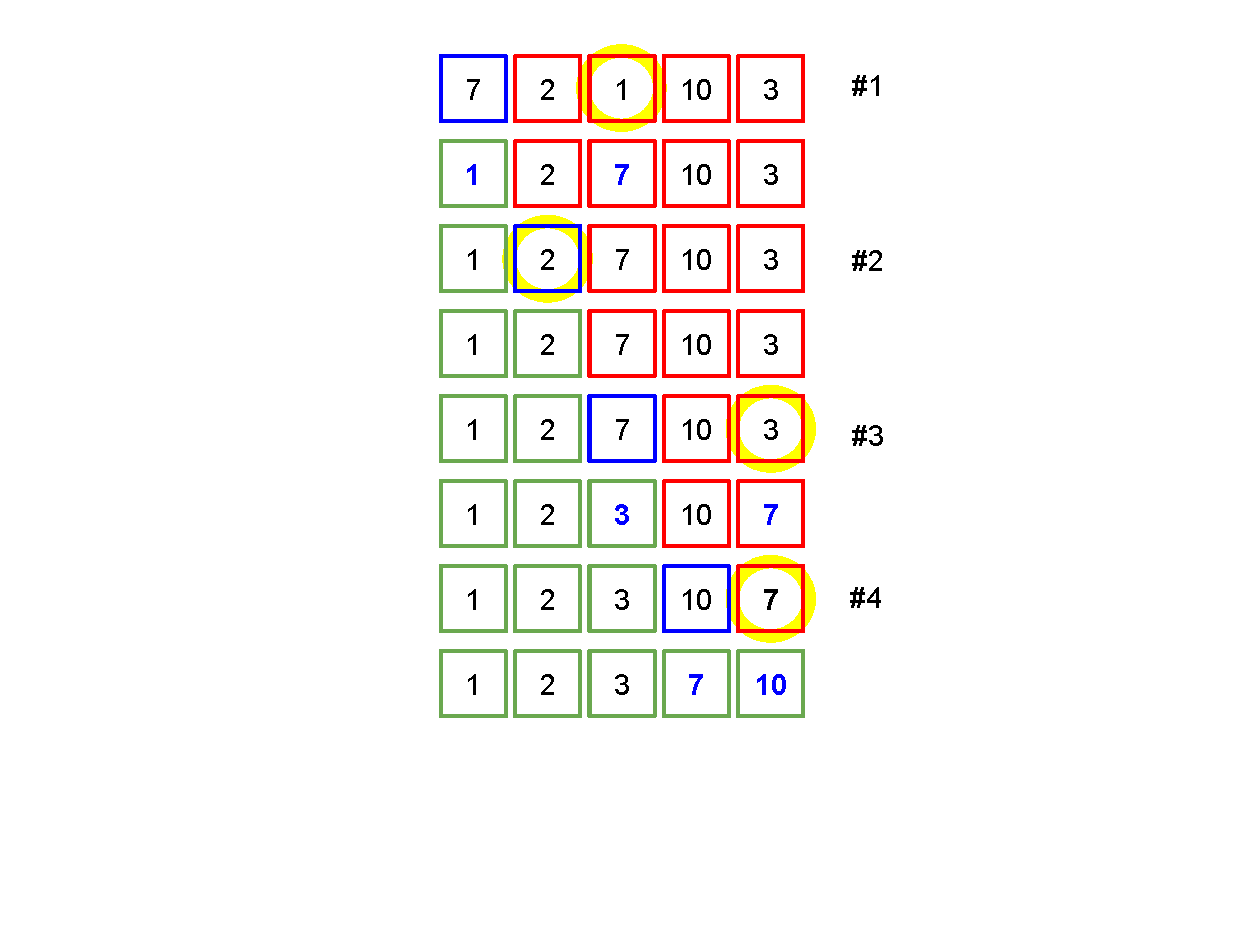
\includegraphics[width=12cm]{images/sssort} 

\end{frame}




\begin{frame}
\centerline{Сортирано сливане / merging}
\end{frame}



\begin{frame}[fragile]
\frametitle{Сортирано сливане / merging}


%\vspace*{-120pt}
%\hspace*{-40pt}
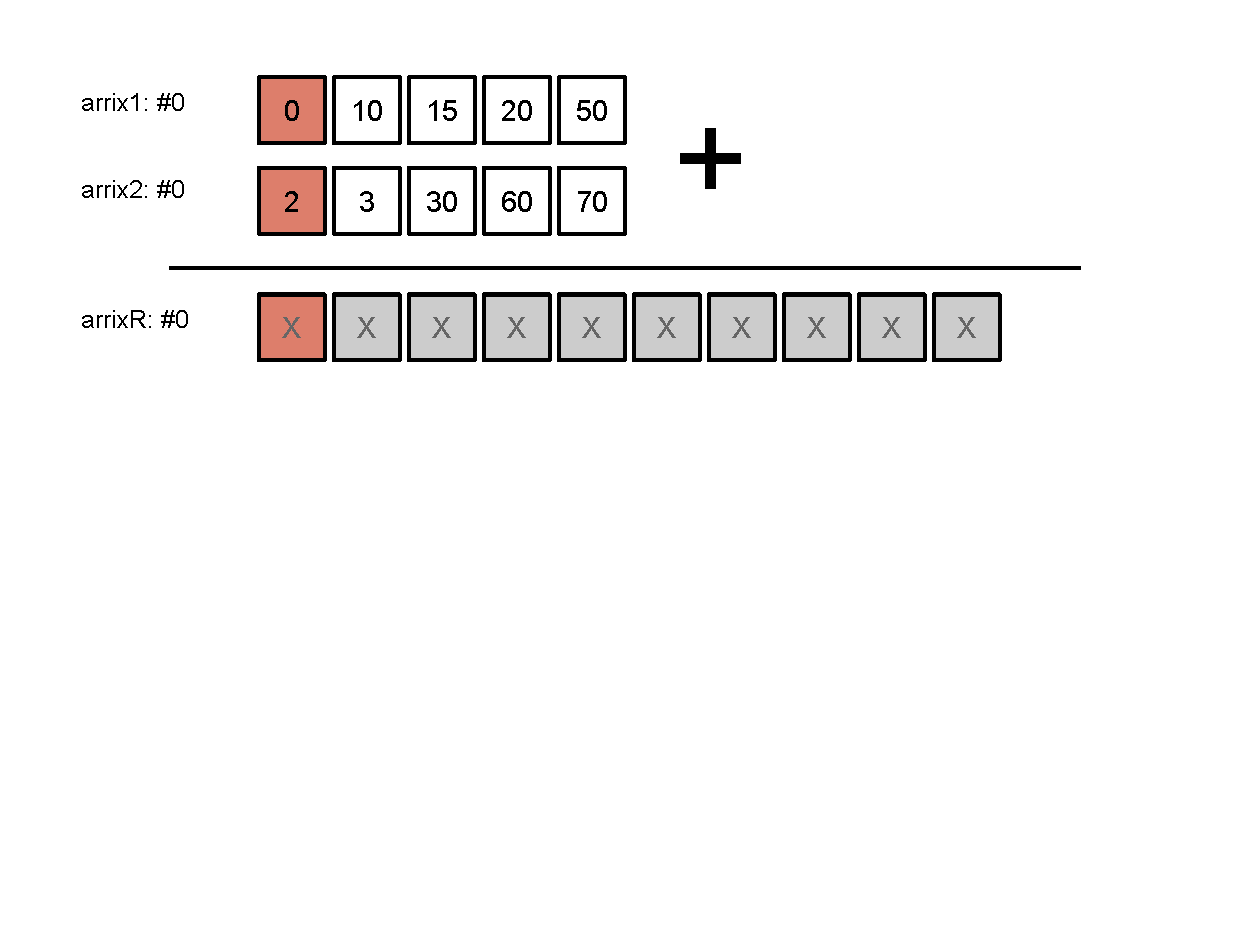
\includegraphics[width=12cm]{images/merge0} 

\end{frame}


\begin{frame}[fragile]
\frametitle{Сортирано сливане / merging}


%\vspace*{-120pt}
%\hspace*{-40pt}
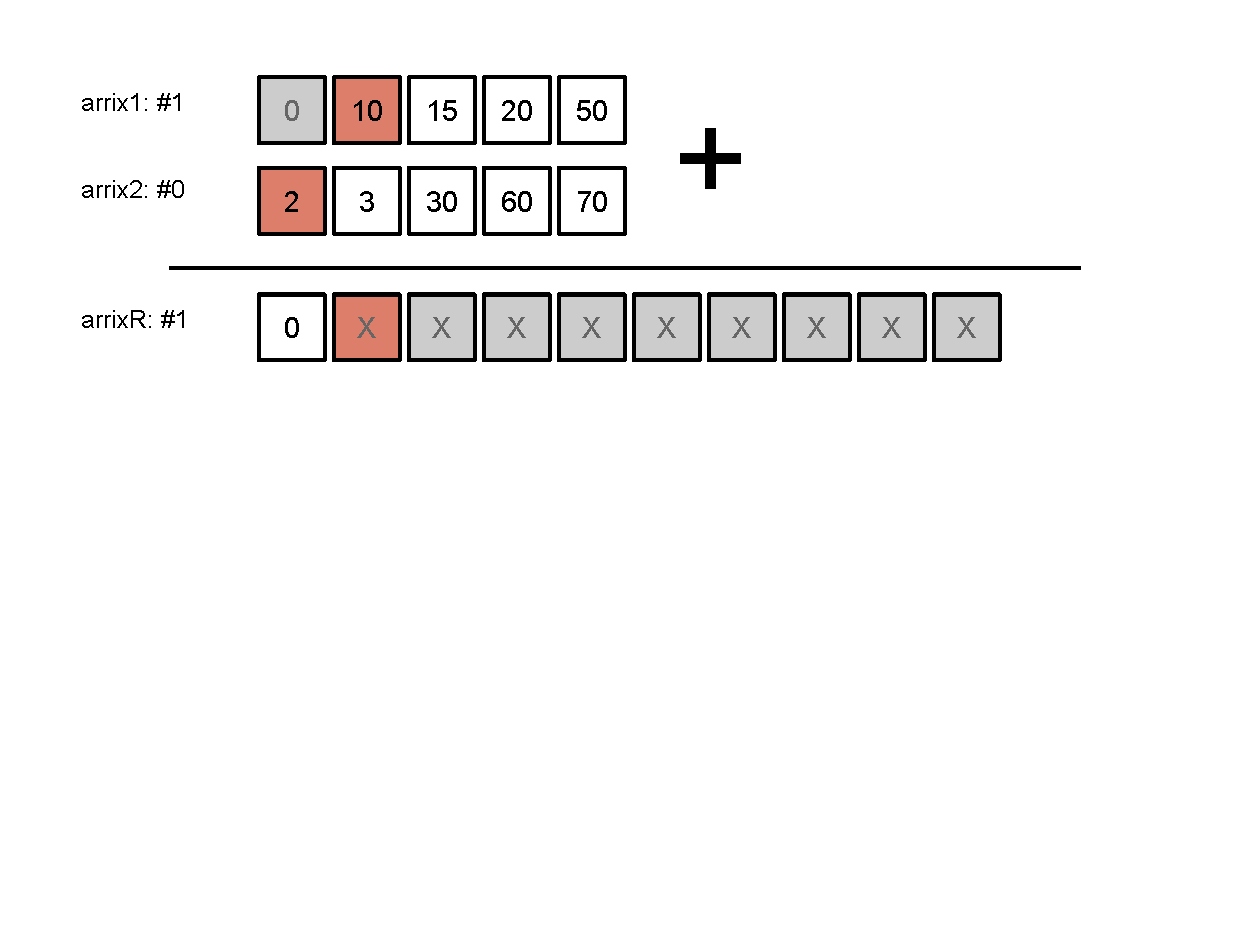
\includegraphics[width=12cm]{images/merge1} 

\end{frame}
\begin{frame}[fragile]
\frametitle{Сортирано сливане / merging}


%\vspace*{-120pt}
%\hspace*{-40pt}
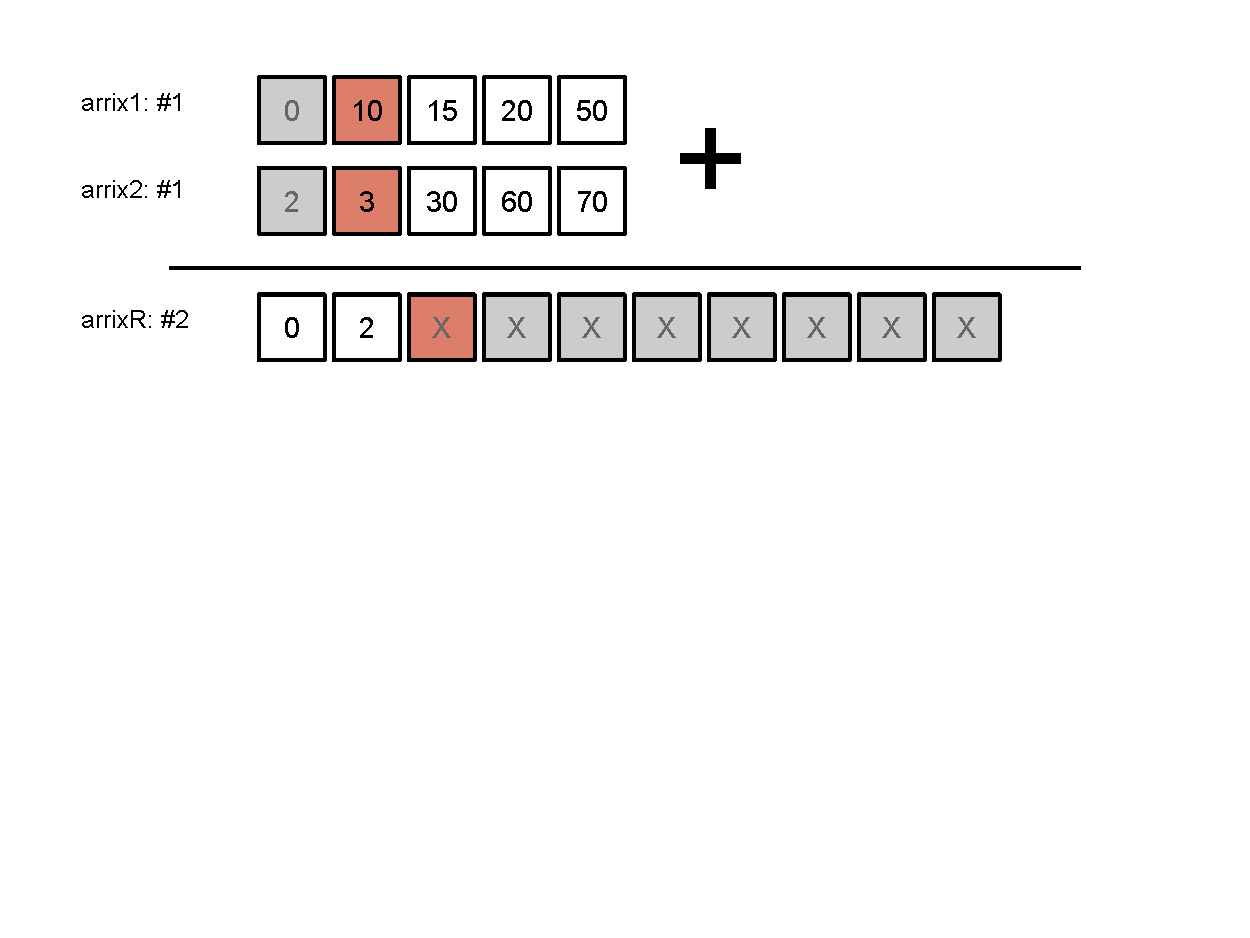
\includegraphics[width=12cm]{images/merge2} 

\end{frame}
\begin{frame}[fragile]
\frametitle{Сортирано сливане / merging}


%\vspace*{-120pt}
%\hspace*{-40pt}
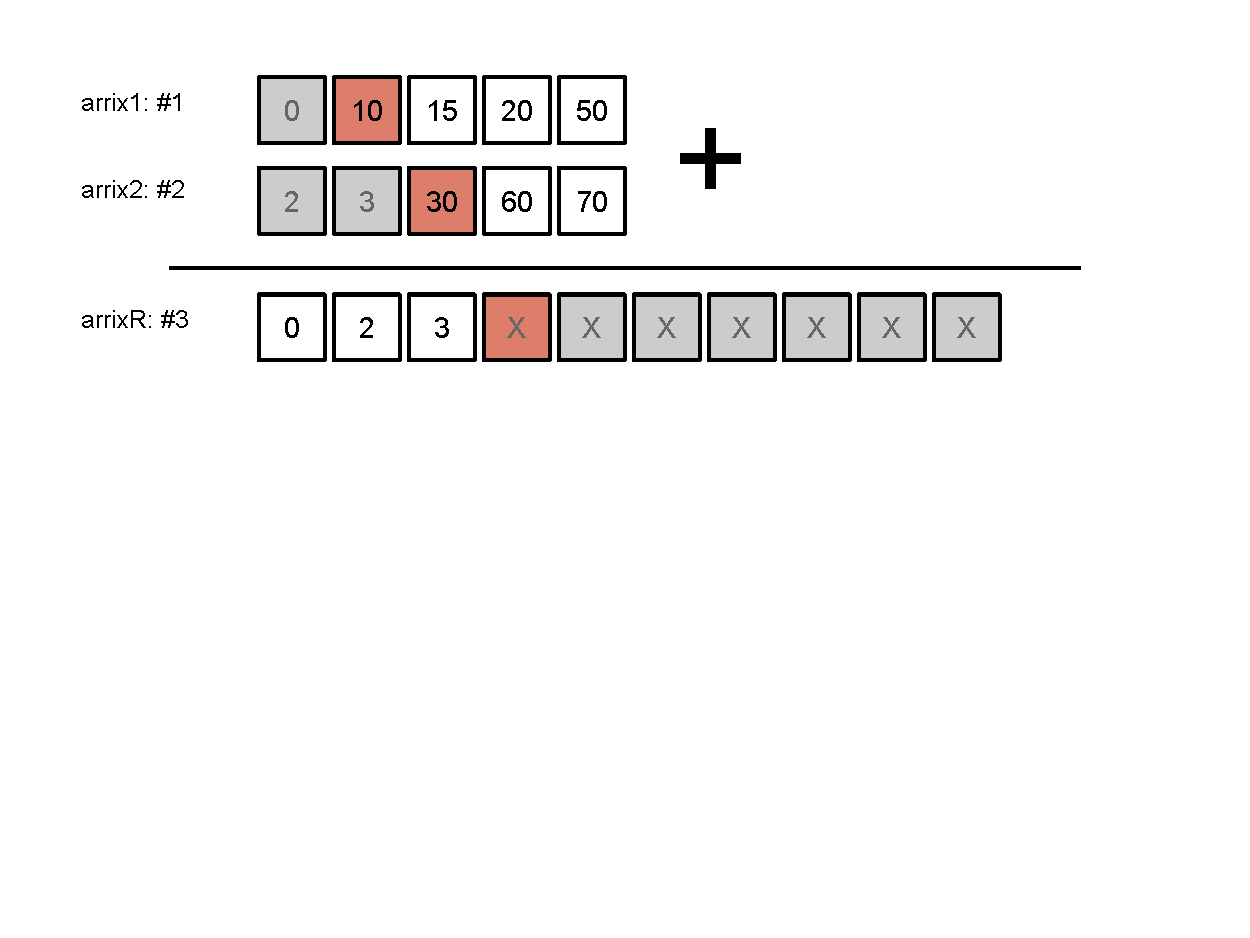
\includegraphics[width=12cm]{images/merge3} 

\end{frame}
\begin{frame}[fragile]
\frametitle{Сортирано сливане / merging}


%\vspace*{-120pt}
%\hspace*{-40pt}
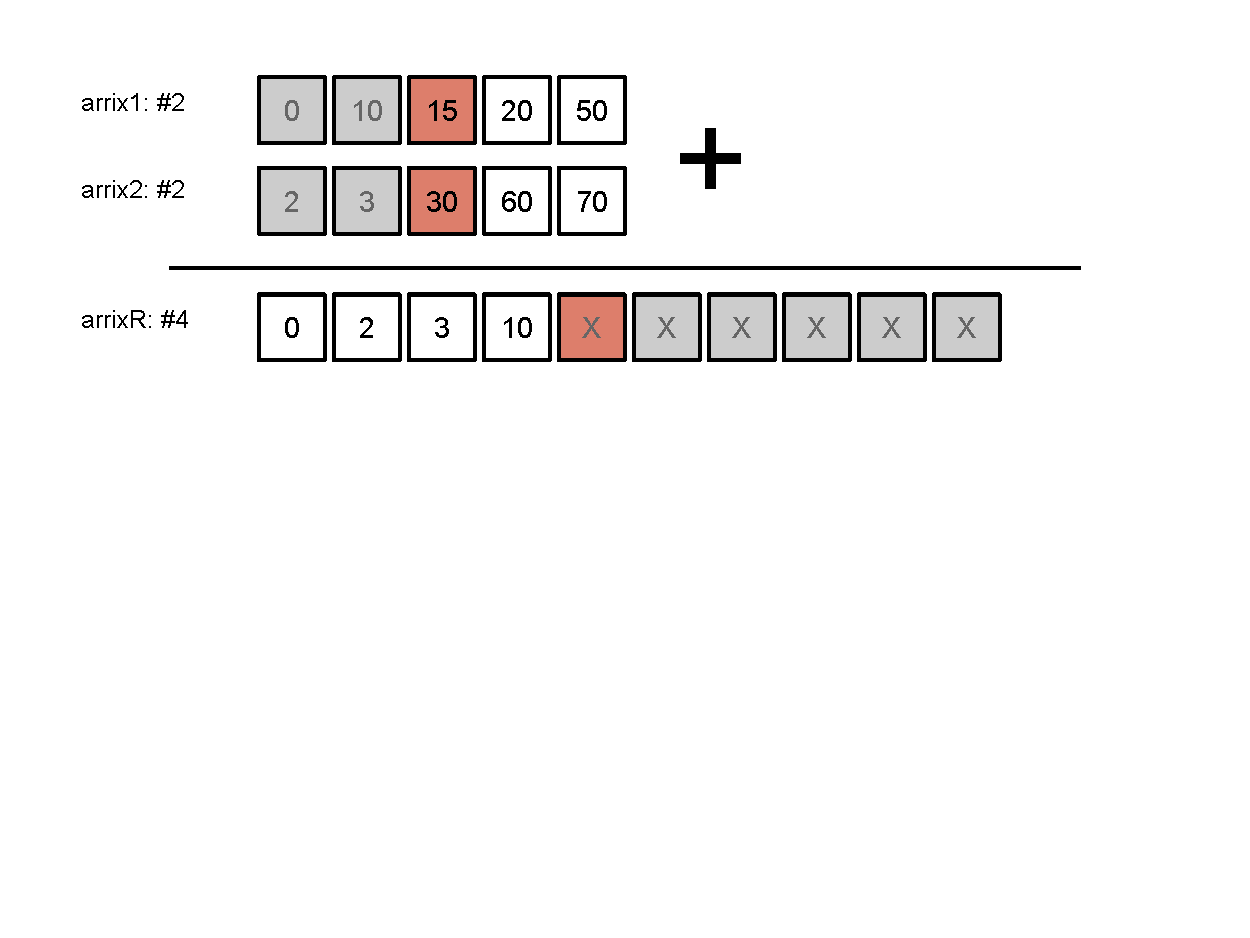
\includegraphics[width=12cm]{images/merge4} 

\end{frame}
\begin{frame}[fragile]
\frametitle{Сортирано сливане / merging}


%\vspace*{-120pt}
%\hspace*{-40pt}
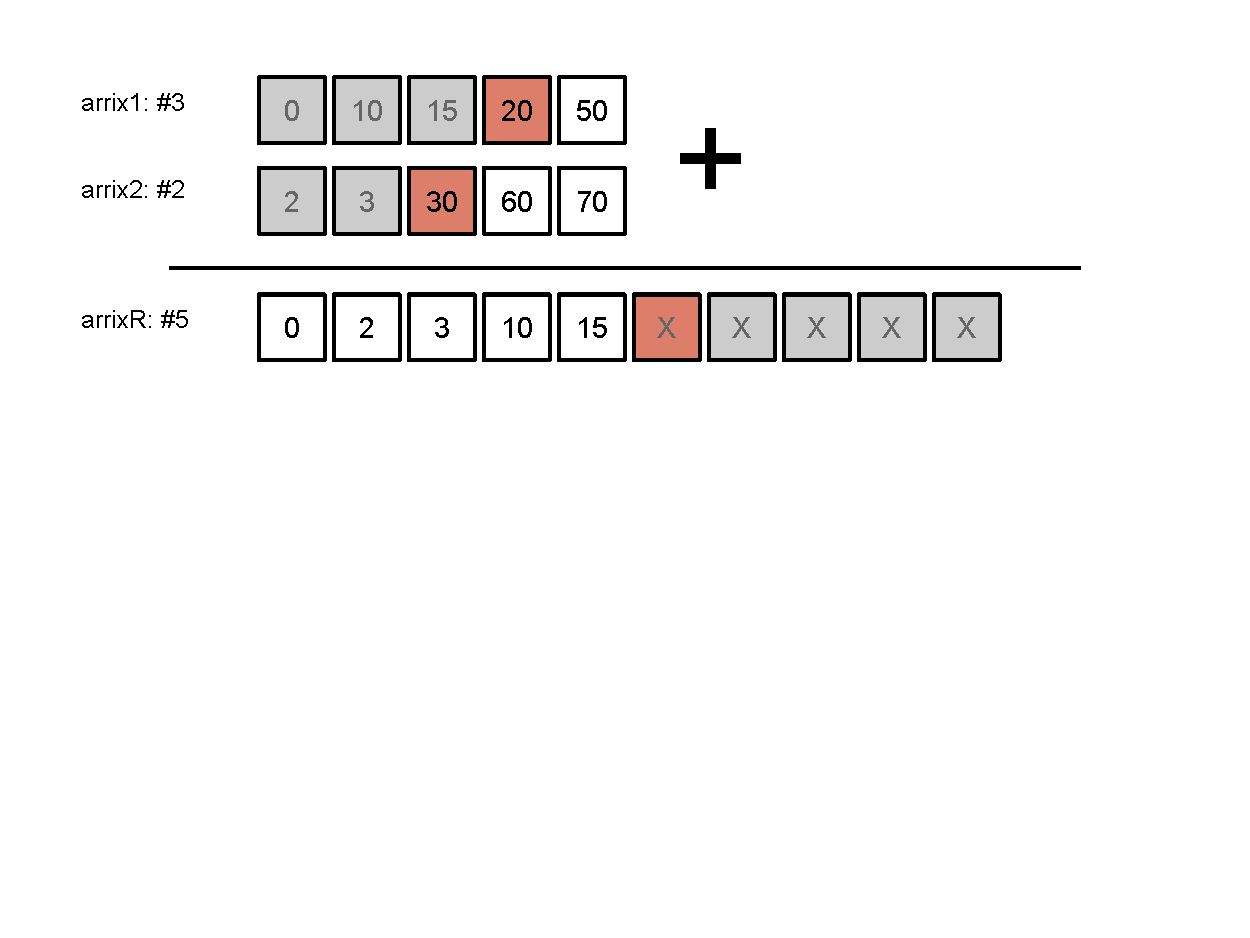
\includegraphics[width=12cm]{images/merge5} 

\end{frame}
\begin{frame}[fragile]
\frametitle{Сортирано сливане / merging}


%\vspace*{-120pt}
%\hspace*{-40pt}
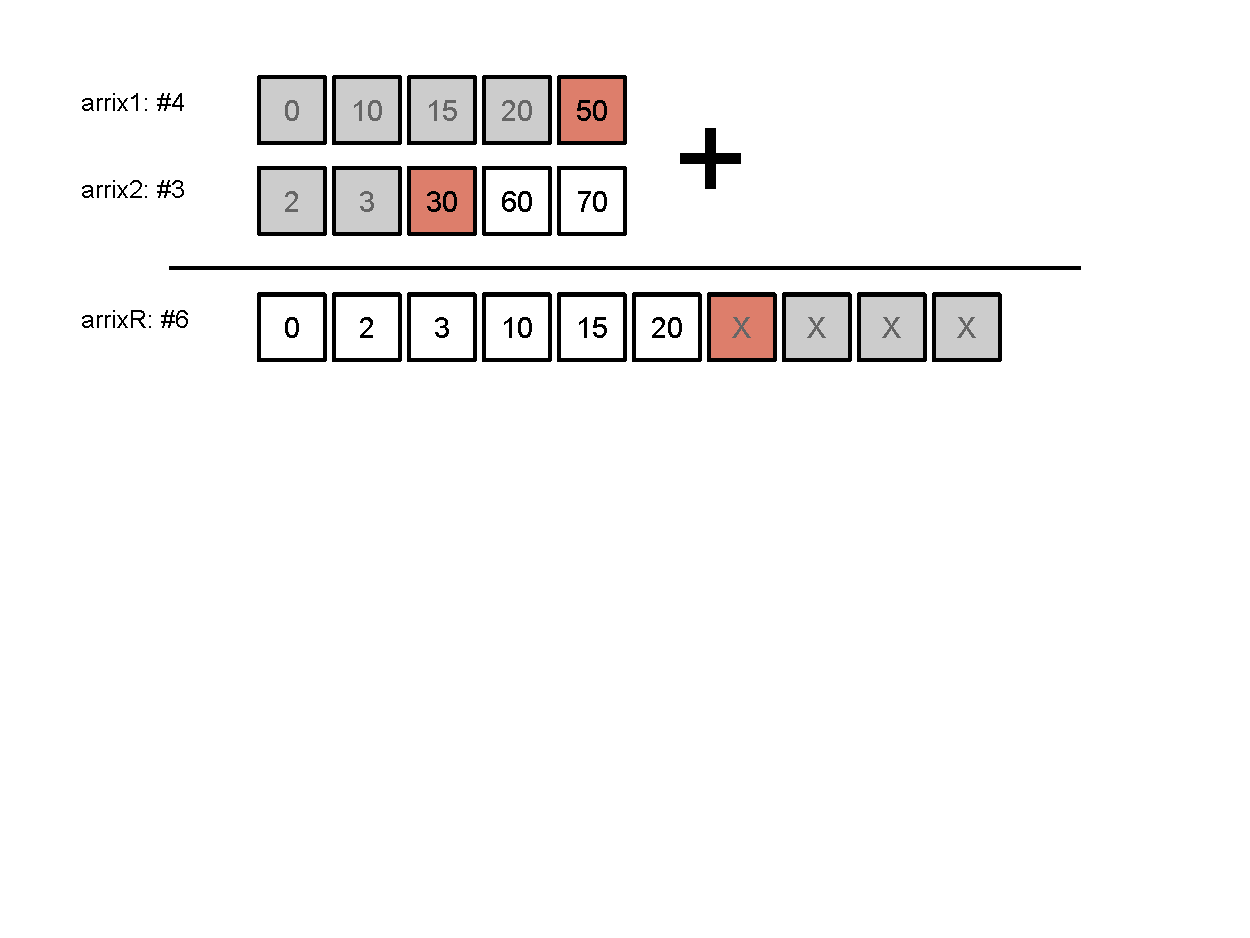
\includegraphics[width=12cm]{images/merge6} 

\end{frame}
\begin{frame}[fragile]
\frametitle{Сортирано сливане / merging}


%\vspace*{-120pt}
%\hspace*{-40pt}
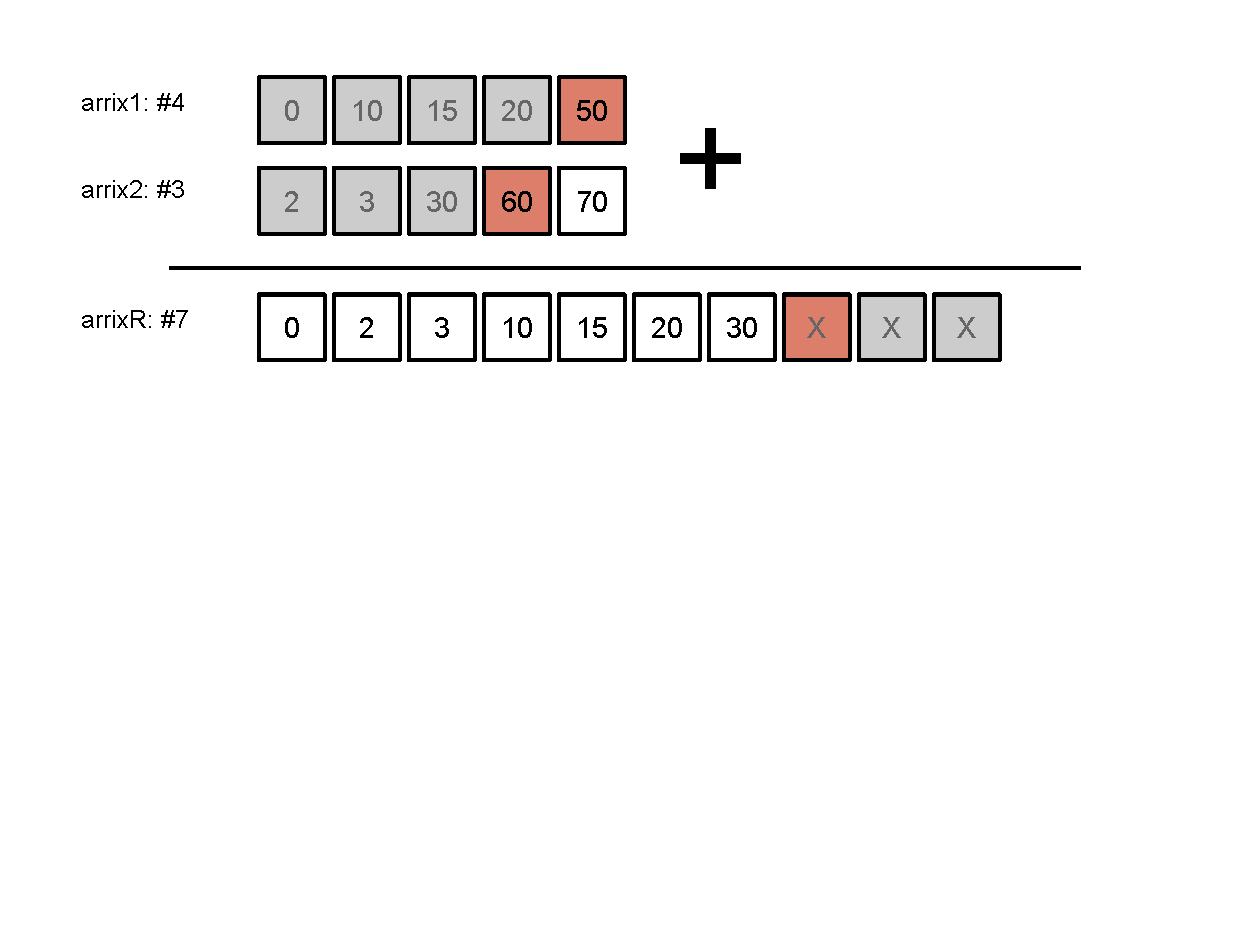
\includegraphics[width=12cm]{images/merge7} 

\end{frame}
\begin{frame}[fragile]
\frametitle{Сортирано сливане / merging}


%\vspace*{-120pt}
%\hspace*{-40pt}
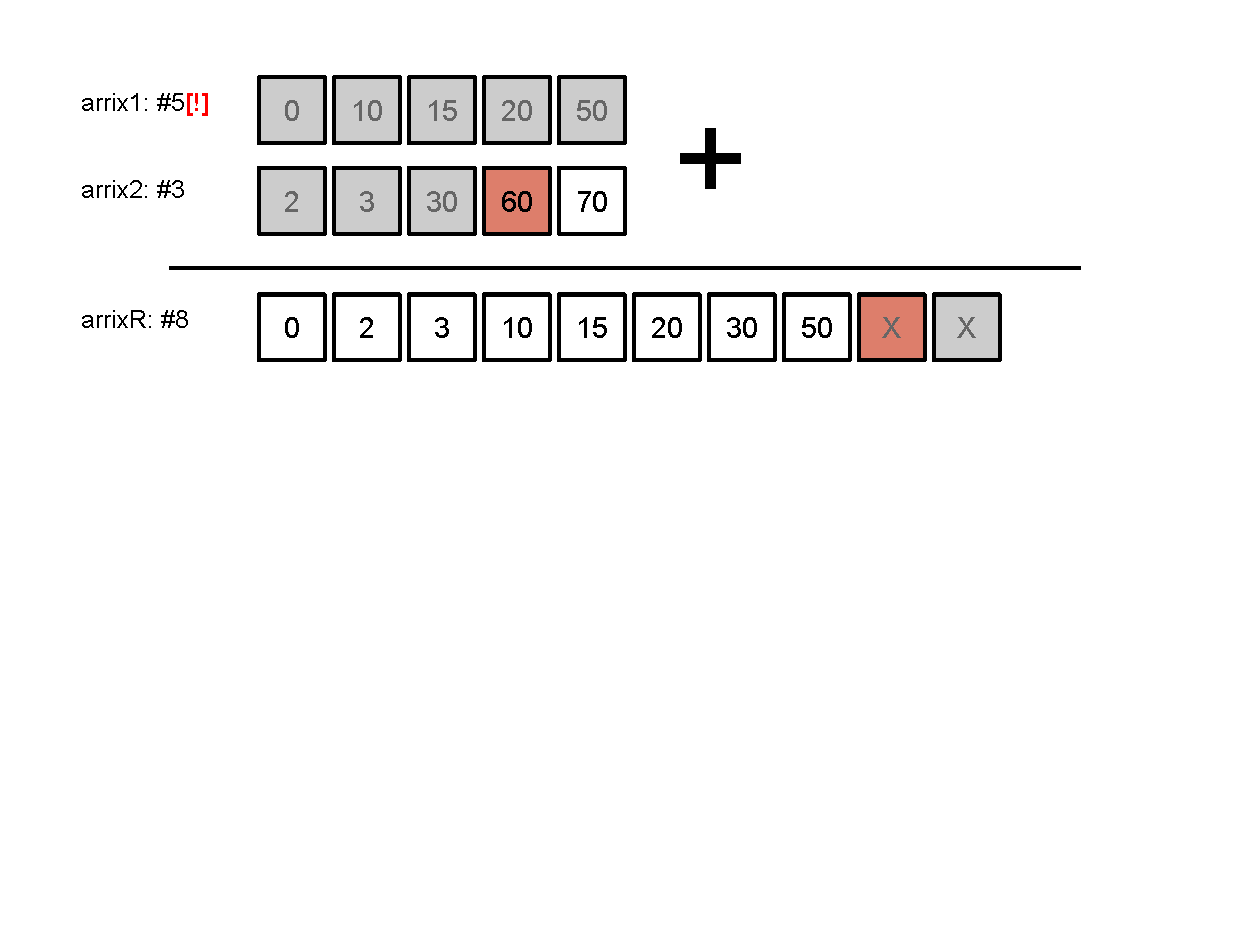
\includegraphics[width=12cm]{images/merge8} 

\end{frame}


\end{document}


\begin{columns}[t]
  \begin{column}{0.2\textwidth}

  \end{column}
  \begin{column}{0.8\textwidth}

  \end{column}
\end{columns}


